\section{Collective Conceptualization (Offline Learning)}
In this section, we elaborate how we estimate $P(a)$ and $P( \langle c_{1},c_{2} \rangle |a)$ from knowledge bases, which is the major task in the offline learning component. As we have claimed, our major idea is collectively conceptualize multiple EAE instances instead conceptualizing each instance independently.
% We also introduce computation of $P(a)$ is another important part of the offline component.

\vspace{-2mm}
\paragraph{Collective Conceptualization ($P( \langle c_{1},c_{2} \rangle |a)$) }
We use SPO triples in DBPedia to compute the probability.
%We use these entity-attribute-entity instances to estimate the conditional probability of a concept pair given an attribute. 
The key of the computation is to assign a larger value for the true concepts pairs than false concept pairs.
For a certain attribute $a_k$, there are many entity pairs connected by the attribute in DBpedia, which allow us to aggregate the support from all entity pairs.
The aggregated score helps identify the true concept pair attribute to these properties:
\begin{enumerate}
\small
\item \emph{A false concept pairs are only supported by quite a few
entity pairs that have the attribute.}
\item \emph{A true concept pair in general is supported by most entity pairs of the attribute.}
\end{enumerate}

More formally, let $ \langle e_i, a_k, e_j \rangle $ be a SPO triple in DBPedia.
%The triple means that entity $e_i$ has a attribute $a_k$ with value or object as $e_j$.
%We only consider the SPO triples with O as entity, this attributes such as \at{height,year} are removed in the first place. 
Let $T_k=\{\langle e_i, a_k, e_j \rangle\}$ be all the triples in DBpedia with attribute as $a_k$.
$P( \langle c_1, c_2 \rangle |a_k)$ is estimated as follows:
\begin{equation}
\small
P(\langle c_1, c_2\rangle|a_k)= \frac{1}{|T_k|}\sum_{  (e_{i},a_k,e_{j})\in T_k } P(c_1|e_{i})P(c_2|e_{j})
\label{eq:pccga}
\end{equation}
It is not difficult to prove that $0\leq P( \langle c_1, c_2 \rangle |a_k)\leq 1$ and their sum over all concept pairs equals to 1.
Hence $P( \langle c_1, c_2 \rangle |a_k)$ is a probability estimation.


{\footnotesize
\begin{example}[Calculating $P( \langle {c_h}_{1},{c_h}_{2} \rangle  |a)$]
\label{exa:pggga}
Figure~\ref{fig:bipartite} shows many entity pairs of attribute \at{FoundedBy}. 
We can see that the false concept such as \at{fruit} is supported by only \at{Steve Jobs}.
However, the true concept pair \at{<company, entrepreneur>} is supported by all the three concept pairs. 
By summing up all $P(c_1|e_1)P(c_2|e_2) $ over all entity pairs, the true concept pair \at{<company, entrepreneur>} has a significant larger score than the false one \at{<fruit, entrepreneur>}.
\end{example}
}


%\vspace{-2mm}
\begin{figure}[!htb]
\vspace{-6mm}
\centering
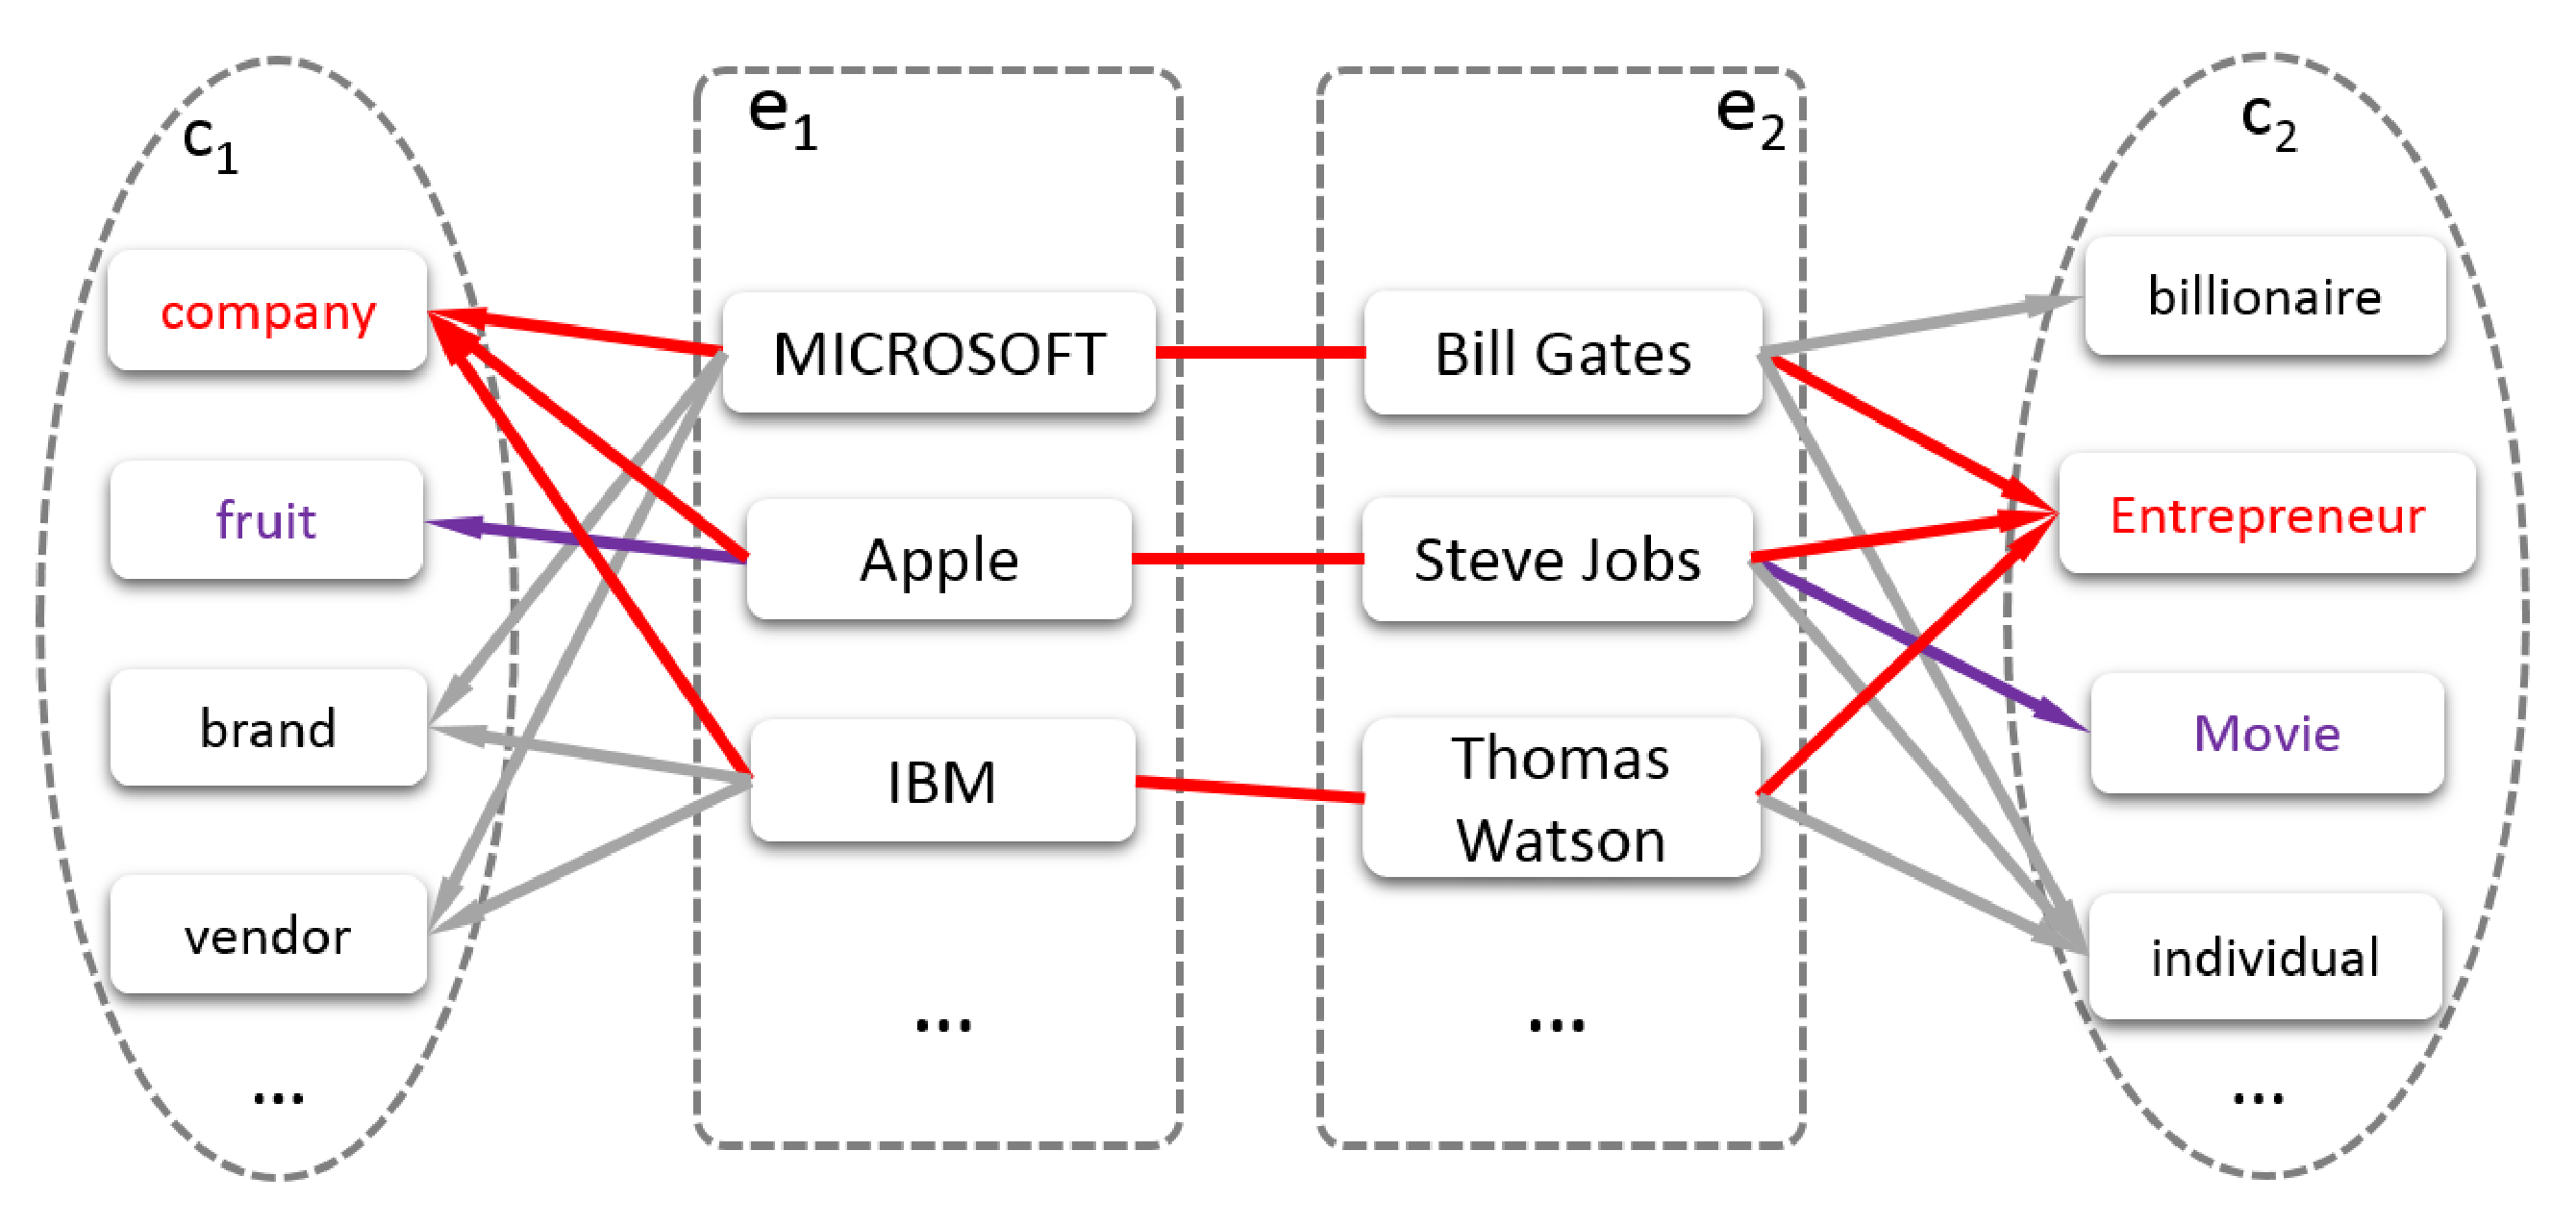
\epsfig{file=resources/ceaec.eps,width=\columnwidth, height=0.4\columnwidth}
\vspace{-8mm}
\caption{Calculating $P(  \langle {c}_{1},{c}_{2} \rangle  | \term{FoundedBy} )$ }
\label{fig:bipartite}
\vspace{-3mm}
\end{figure}

\vspace{-2mm}
\paragraph{Computation of $P(a)$}
For a given attribute $a$, $P(a)$ can be computed by
$
P(a)=\frac{n(a)}{\sum_{a_k\in A}{n(a_k)}},
$
where $n(a)$ is the count of triples in DBpedia with attribute $a$.
Note that only we only use SPO triples where both S and O are entities.


%\nop{
%\paragraph{Complexity analysis}
%
%We first analysis the complexity of calculating $P(\langle c_i, c_j \rangle|a_k)$, manifest in Table.~\ref{tab:complexity}. The original one need to calculate $P(\langle c_i, c_j \rangle|a_k)$ for all $c \in C_1,C_2 $,while most of the concepts are, according to the power law, close to zero, which indicates the rationality of pruning.
%
%
%\begin{table}[htbp]
%  \centering
%  \caption{Complexity Analysis}
%    \begin{tabular}{rr}
%    \toprule
%    method & complexity \\
%    \midrule
%    original &  $O(|T_n||C_1||C_2|)$ \\
%    topKpruned & $O(|T_n|K^2)$ \\
%    \bottomrule
%    \end{tabular}%
%  \label{tab:complexity}%
%\end{table}%
%}






%%% Local Variables:
%%% mode: latex
%%% TeX-master: "main.tex"
%%% End:
